\documentclass{ximera}

%\newtheorem{theorem}{Theorem}%[section] % reset theorem numbering for each section
%\newtheorem*{theorem*}{Theorem}%[section] % reset theorem numbering for each section
%\newtheorem{prop}[theorem]{Proposition}
%\newtheorem{lem}[theorem]{Lemma}
%\newtheorem{ex}{Example}


\title{April 20--Farey sequence}  
\begin{document}  
\begin{abstract}  We explore the Farey sequence of rational numbers.
\end{abstract}  
\maketitle  

There are several equivalent ways of defining successive Farey sequences. We will show that these are equivalent, as well as prove some properties of these sequences.

\begin{definition}
 The \emph{level $n$ Farey fractions} \emph{between $0$ and $1$}  is the set of reduced form fractions ordered from smallest to largest with
 \[S_n=\left\{\frac{p}{q}:0\leq \frac{p}{q}\leq 1, (p,q)=1, 1\leq q  \leq n\right\}.\] So that every term in the sequence is a fraction, we write $0=\frac{0}{1}$  and $1=\frac{1}{1}$.  The first four Farey sequences are 
\begin{align*}
 S_1&=\left\{\frac{0}{1},\frac{1}{1}\right\}\\
 S_2&=\left\{\frac{0}{1},\answer{\frac{1}{2}},\frac{1}{1}\right\}\\
 S_3&=\left\{\frac{0}{1},\answer{\frac{1}{3}},\answer{\frac{1}{2}},\answer{\frac{2}{3}},\frac{1}{1}\right\}\\
 S_4&=\left\{\frac{0}{1},\answer{\frac{1}{4}},\answer{\frac{1}{3}},\answer{\frac{1}{2}},\answer{\frac{2}{3}},\answer{\frac{3}{4}},\frac{1}{1}\right\}\\
\end{align*}
\end{definition}
%To keep the two definitions straight, we refer to the $n^{th}$ Farey sequence from this definition as $F_n$, and the $n^{th}$ row of the table in the second definition as $f_n$.
It is clear that each sequence $S_n$ is ordered from smallest to largest and that each $(p,q)=1$ (since these facts are both part of the definition). 
However, these facts are less obvious for the next definition, $f_n$:

\begin{definition}
 Construct a table using the following rules: In the first row, write $\frac{0}{1}$ and $\frac{1}{1}$. 
 
For the $n^{th}$ row, copy the $(n-1)^{st}$ row. For each $\frac{a}{b}$ and $\frac{c}{d}$ in the$(n-1)^{st}$ row, insert $\frac{a+c}{b+d}$ between $\frac{a}{b}$ and $\frac{c}{d}$ if $b+d\leq n$.
The first four rows are 
\begin{tabular}{cccccccc}
$f_1$&$\frac{0}{1}$&&&&&&$\frac{1}{1}$\\
$f_2$&$\frac{0}{1}$&&&$\answer{\frac{1}{2}}$&&&$\frac{1}{1}$ \\
$f_3$&$\frac{0}{1}$&&$\answer{\frac{1}{3}}$&$\answer{\frac{1}{2}}$&$\answer{\frac{2}{3}}$&&$\frac{1}{1}$ \\
$f_4$&$\frac{0}{1}$&$\answer{\frac{1}{4}}$&$\answer{\frac{1}{3}}$&$\answer{\frac{1}{2}}$&$\answer{\frac{2}{3}}$&$\answer{\frac{3}{4}}$&$\frac{1}{1}$
\end{tabular}

We call the sequence in the $n^{th}$ row of the table $f_n$.
\end{definition}

It is clear that for each $\frac{a}{b}$ and $\frac{c}{d}$ in the$(n-1)^{st}$ row, we insert $\frac{a+c}{b+d}$ between $\frac{a}{b}$ and $\frac{c}{d}$ if $b+d\leq n$ (since this is the definition). This unusual (but easier) way of adding fractions gives what we call \emph{median convergents}.

We are going to prove that $f_n=S_n$ for every $n$;  that the $n^{th}$ row of the table consists of all $\frac{p}{q}$ with $0\leq \frac{p}{q}\leq 1, (p,q)=1, 1\leq q  \leq n$; and that the fractions in each row are ordered from smallest to largest. From there, we get that for each $\frac{a}{b}$ and $\frac{c}{d}$ in the  $F_{n-1}$, we insert $\frac{a+c}{b+d}$ between $\frac{a}{b}$ and $\frac{c}{d}$ if $b+d\leq n$ 

In both definitions, if $\frac{a}{b}$ and $\frac{c}{d}$ are next to each other in $S_n$ (or $f_n$), then we say they are \emph{consecutive fractions in $S_n$ (or $f_n$)}.

\begin{theorem}[Textbook Theorem 6.1]
 If $\frac{a}{b}$ and $\frac{c}{d}$ are consecutive fractions in $f_n$ with $\frac{c}{d}$ to the left of $\frac{a}{b}$, then $ad-bc=1$.
\end{theorem}
\begin{proof}
 We use induction. For $n=1$, there are only two fractions, and $1(1)-0(1)=1$.
 
 Assume that this fact holds for the $(n-1)^{st}$ row. That is, $ad-bc=1$ for all $\frac{a}{b}$ and $\frac{c}{d}$ consecutive Farey fractions in $F_{n-1}$ with $\frac{c}{d}<\frac{a}{b}$. For each pair, there are two options for the $n^{th}$ row: either $b+d>n$, so $\frac{a}{b}$ and $\frac{c}{d}$ are still consecutive Farey fractions or $b+d\leq n$, so $\frac{a}{b},\frac{a+c}{b+d}$ and $\frac{c}{d}$ are consecutive Farey fractions. If $b+d>n$, we are done. If $b+d\leq n$, then $\frac{c}{d},\frac{a+c}{b+d},$ and $\frac{a}{b}$ are consecutive fractions, and we need to check both new pairs.
\begin{align*}
 (a+c)d-(b+d)c&=ad+cd-bc-cd\\
 &=ad-bc=1 \quad\textrm{ (by induction hypothesis)}\\
 a(b+d)-b(a+c)&=ab+ad-ba-cb\\
 &=ad-bc=1 \quad\textrm{ (by induction hypothesis)}
\end{align*}
\end{proof}

\begin{corollary}[Textbook Corollary 6.2]
 Every $\frac{p}{a}$ in the table is in reduced form, ie, $(p,q)=1$
\end{corollary}

\begin{corollary}[Textbook Corollary 6.3]
The fractions in each row are ordered from smallest to largest.
\end{corollary}

\begin{theorem}[Textbook Theorem 6.4]
 If $\frac{a}{b}$ and $\frac{c}{d}$ are consecutive fractions in any row, then for all $f_n$ that contain $\frac{a+c}
 {b+d}$, $\frac{a+c}{b+d}$ has the smallest denominator of any rational number between $\frac{a}{b}$ and $\frac{c}{d}$ and is the unique rational number between $\frac{a}{b}$ and $\frac{c}{d}$ with denominator $b+d$.
 \end{theorem} 
 
\begin{proof}
 From the definition, $\frac{a+c}{b+d}$ is the first fraction to appear between $\frac{a}{b}$ and $\frac{c}{d}$ in row $b+d$. Thus, $\frac{c}{d}<\frac{a+c}{b+d}<\frac{a}{b}$ by Corollary 6.3. Now consider any $\frac{x}{y}$ with $\frac{c}{d}<\frac{x}{y}<\frac{a}{b}$. Then 
 \begin{align*}\frac{a}{b}-\frac{c}{d}&=\left(\frac{a}{b}-\frac{x}{y}\right)+\left(\frac{x}{y}-\frac{c}{y}\right)\\
 &=\frac{ay-bx}{by}+\frac{xd-cd}{dy}\geq \frac{1}{by}+\frac{1}{dy}=\frac{b+d}{bdy}
 \end{align*}
 and thus \[\frac{b+d}{bdy}\leq \frac{ad-bd}{bd}=\frac{1}{bd}\] and $y\geq b+d$. If $y>b+d$, then $\frac{x}{y}$ does not have the least denominator of rational numbers between $\frac{a}{b}$ and $\frac{c}{d}$. If $y=b+d$, then $\frac{ay-bx}{by}+\frac{xd-cy}{dy}= \frac{1}{by}+\frac{1}{dy}$ and $ay-bx=xd-cy=1$. By solving, we find $x=a+c$ and $y=b+d$, so $\frac{x}{y}=\frac{a+c}{b+d}$.
\end{proof}

\begin{theorem}[Textbook Theorem 6.5]
If $0\leq x\leq y, (x,y)=1$, then the fraction $\frac{x}{y}$ appears in the $y^{th}$ row of the table and all future rows.
\end{theorem}
\begin{proof}
 The theorem is true by definition for $y=1$. Assume that the theorem is true for $y=y_0-1$, with $y_0>1$. Then if $y=y_0-1$, then the fraction $\frac{x}{y}$ cannot be in the $(y-1)^{st}$ row by definition. Then $\frac{c}{d}<\frac{x}{y}<\frac{a}{b}$ for some $\frac{a}{b}, \frac{c}{d}$ in the $(y-1)^{st}$ row. Since $\frac{c}{d}<\frac{a+c}{b+d}<\frac{a}{b},$ and  $\frac{a}{b}, \frac{c}{d}$ are consecutive fractions, $\frac{a+c}{b+d}$ is not in the $(y-1)^{st}$  row. Thus $b+d>y-1$ by the induction hypothesis. By Theorem 6.4, $y\geq b+d$, so $y=b+d$. By the uniqueness part of Theorem 6.4, $x=a+c$. Thus, $\frac{x}{y}$ appears in the $y^{th}$ row of the table and all future rows.
\end{proof}

\begin{corollary}[Textbook Corollary 6.6]
 The $n^{th}$ row consists of all reduce fractions with $\frac{a}{b}$ such that $0\leq \frac{a}{b}\leq 1$ and $0<b\leq n$. The fractions are listed from smallest to largest.
\end{corollary}

Now we have the definition of the Farey sequences which contain the level $n$ Farey fractions between $0$ and $1$.
\begin{definition}
 The $n^{th}$ Farey sequence 
 \[F_n=\left\{\frac{p}{q}:(p,q)=1, 1\leq q  \leq n\right\}.\] So that every term in the sequence is a fraction, we write $n=\frac{n}{1}$.  The first four Farey sequences are 
\begin{align*}
 F_1&=\left\{\dots,-\frac{1}{1},\frac{0}{1},\frac{1}{1},\dots\right\}\\
 F_2&=\left\{\dots,-\frac{1}{1},-\answer{\frac{1}{2}},\answer{\frac{0}{1}},\answer{\frac{1}{2}},\frac{1}{1},\dots\right\}\\
 F_3&=\left\{\dots,-\frac{1}{1},-\answer{\frac{2}{3}},-\answer{\frac{1}{2}},-\answer{\frac{1}{3}},\answer{\frac{0}{1}},\answer{\frac{1}{3}},\answer{\frac{1}{2}},\answer{\frac{2}{3}},\frac{1}{1},\dots\right\}\\
 F_4&=\left\{\dots,-\frac{1}{1},-\answer{\frac{3}{4}},-\answer{\frac{2}{3}},-\answer{\frac{1}{2}},-\answer{\frac{1}{3}},-\answer{\frac{1}{4}},\answer{\frac{0}{1}},\answer{\frac{1}{4}},\answer{\frac{1}{3}},\answer{\frac{1}{2}},\answer{\frac{2}{3}},\answer{\frac{3}{4}},\frac{1}{1},\dots\right\}\\
\end{align*}
\end{definition}
Depending on the source, Farey sequences may or may not be restricted to the interval $[0,1]$. However, if you look at the sets $f_n=S_n$, they aren't really sequences since they are finite.

\begin{remark}
If $\frac{p}{q}=[a_0;a_1,a_2,\dots,a_n]$ with $(p,q)=1$, then the fractions on either side of $\frac{p}{q}$ in the $q^{th}$ Farey sequence are $[a_0;a_1,a_2,\dots,a_n-1]$ and $[a_0;a_1,a_2,\dots,a_{n-1}]$. For example, $\frac{2}{9}$ has continued fraction expansion $[\answer{0};\answer{4},\answer{2}]$ and fractions on either side of $\frac{2}{9}$ in the $9^{th}$ Farey sequence are $\answer{\frac{1}{5}}=[\answer{0};\answer{4},\answer{1}]$ (smaller) and $\answer{\frac{1}{4}}=[\answer{0};\answer{4}]$ (larger).
\end{remark}

The following great image from Wikipedia highlights successive Farey fractions connected by semicircles. $F_1$ in brown, $F_2$ in red, $F_3$ in yellow, etc (the arc from $0$ to $\frac{1}{n}$ tells you the color of the $n^{th}$ Farey sequence). If you view the image on Wikipedia, hovering over a curve to highlights it and the terms in that Farey sequence (this seems to require a desktop browser) \url{https://upload.wikimedia.org/wikipedia/commons/9/91/Farey_diagram_horizontal_arc_9.svg}
\begin{image}
 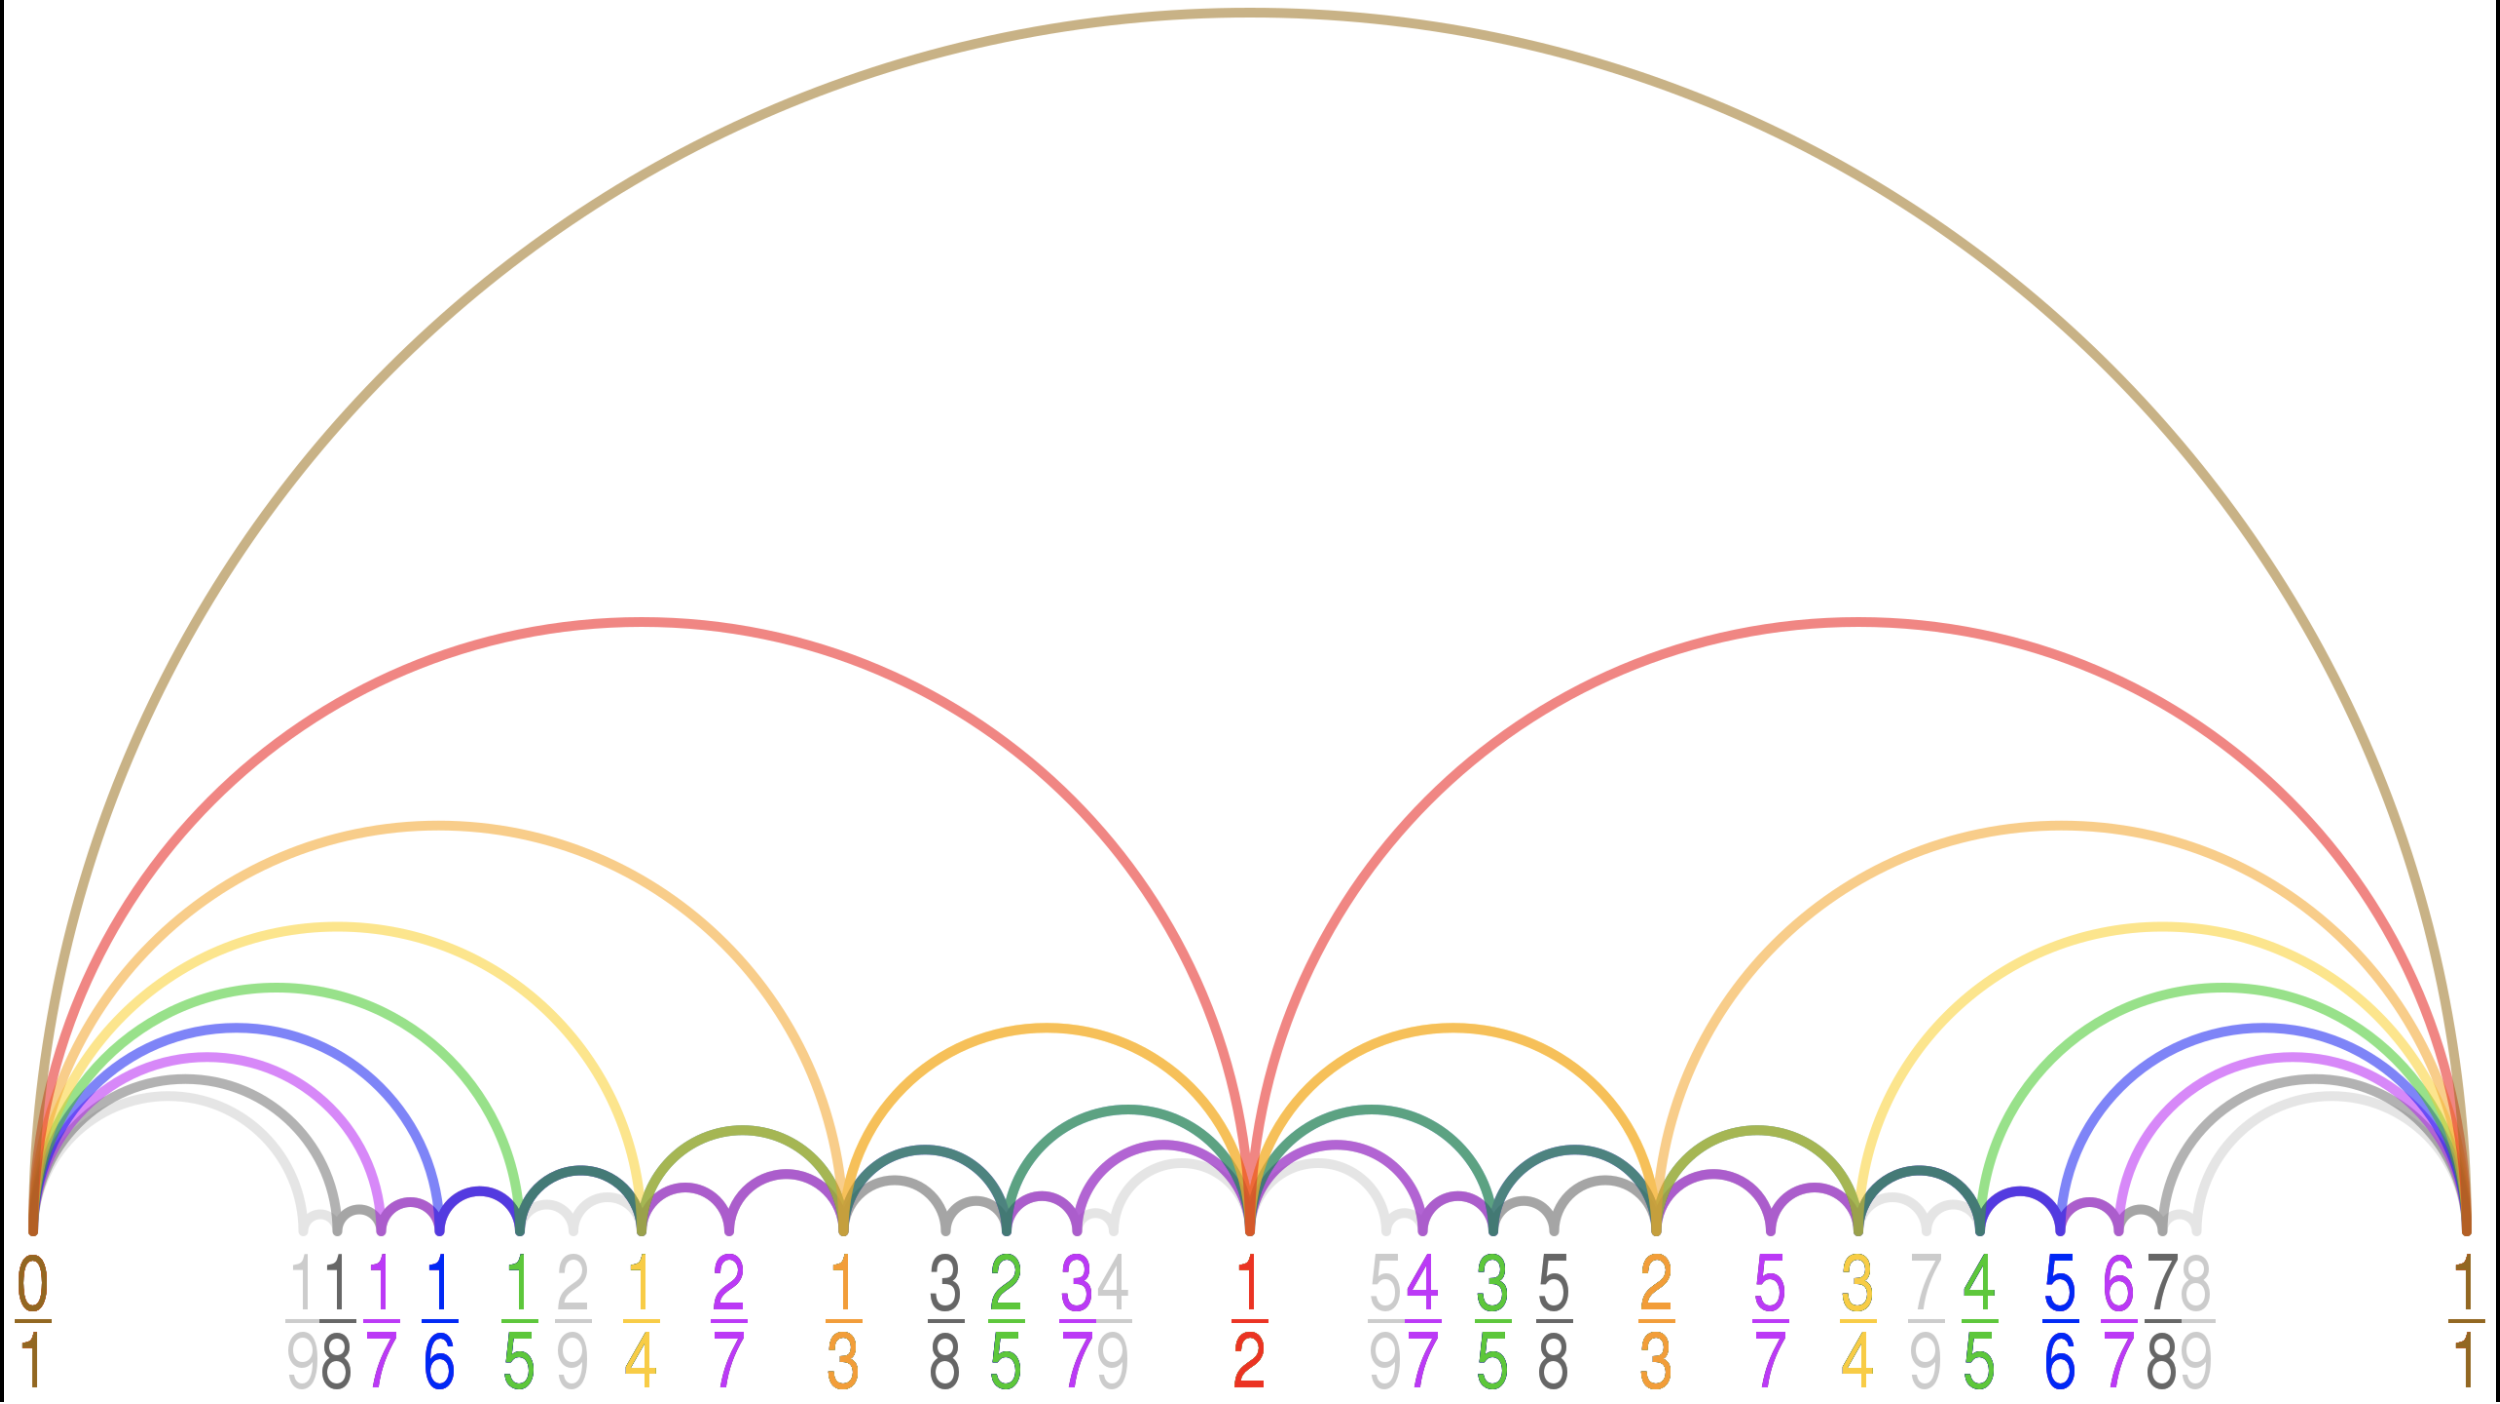
\includegraphics{farey}
\end{image}
\end{document}